\chapter{Architecture and implementation of the Journal and Stream Processing part}

\section{Architecture}

As presented in the Requirements chapter, the Journal needs to store the events as an append-only list. The Journal should also provide a way for stream processors to subscribe to the real-time stream of events. Stream processors can subscribe to themselves in a Tree-like structure (see Figure \ref{fig:tree}), and upon the reception of an event a processor can create a substream of events and perform side-effects.
\\

\subsection{Naive push-only solutions}

An important problem that will solve the architecture is the fact that the Journal can have an event stream rate that is superior to its subscribers. More generally,
any parent node (Journal or processor) can have an output stream rate that is superior to the event processing time of one or several of its children. 
Several simple \textit{push} solutions can be applied, but none of them were applicable for our system.

First, any child can just have an in-memory buffer that stores the incoming events not yet processed. However, an in-memory buffer has obvious limitations like causing an OutOfMemory exception if the child can not handle the flow rate and start queuing a lot of events. Moreover, as said in the non-functional requirements part, one goal is to limit the RAM consumption of the platform. Thus, this solution is not applicable.

Another solution can be for a parent node to wait that all its children have processed the current event to send the next one via an ACK mechanism. 
An obvious issue of this approach is that
the slowest child of a parent will slow down the event stream rate for all its siblings. This is clearly not acceptable for a scalable system with loose coupling 
between components. Moreover, such a solution implies that the failure of a child stops the stream for its siblings, which is clearly not a fault-tolerant approach.

As a reminder, no message loss is a requirement for the platform, so dropping the events if the stream rate is too fast is not an option.
\\

\subsection{Pull-based streaming with event-sourced processors}

One suitable solution is to use a pull-model instead of a push-model. For each received event, a processor processes it to produce a substream and stores the events of this substream in a local journal as a side-effect. Thus, each processor maintains its own event journal, so each processor is \textit{event-sourced}.
This allows each child to maintain a cursor on the journal of its parent pointing on the next event to pull. Thus, children can have totally different pulling and processing speeds, they are not coupled to each other. This approach of pull-based stream systems with decoupled multi-consumers using cursors comes from Apache Kafka, a distributed messaging system for log processing created at LinkedIn \footfullcite{bib:kafka}. 

A common problem with pull-based system is the polling part. How can children know when the next event is ready to be pulled? The naive way to do this is to check every X seconds / milliseconds if the parent has a new event in its journal. This can waste a lot of resources when a parent has no new event for a while. The solution brought by Kafka is to 
perform long-polling: when the child's cursor goes on the next event, either it pulls this next event if it exists or it blocks until a new event comes in to pull it. Thus, children do not have to pull periodically to know whether there is a new event.

However, the term "blocks" does not really get along well with our reactive non-blocking architecture. We therefore have to find a way to implement long-polling without blocking
threads. To do that, we will use the Promise abstraction described in section \ref{sec:promises}. Mixing Futures, Iteratees and Promises, we will be able to implement
an asynchronous non-blocking long-polling system (more details in the Implementation section \ref{sec:streamimplementation}).

Both the Journal and the local journals of processors are persistent using MongoDB. MongoDB is a document-oriented NoSQL database \footfullcite{bib:mongodb} that stores BSON documents (a binary representation of JSON). The format of stored event is a BSON-serialized version of ZEvents (see Listing \ref{lst:zevent}). It contains an id, the name of the resource (for example \verb|/resourceType1/id4|), the user that inserted the event in the Journal, the insertion date, the type of event and the body (data) of the event in a JSON object. To model a journal, we just use a MongoDB collection where we only insert new documents (events). To keep the insertion order of events, an id of type PathId is serialized
into the document. MongoDB provides a built-in id generation mechanism that keeps the insertion order, but the fact of ensuring message ordering of \textit{substream} across processors implies to create a more sophisticated id generation mechanism. This will be explained thoroughly in section \ref{sec:substreamproblem}.
\\

Thus, each event produced by a processor goes into its MongoDB local journal, and children pull events (one by one or by bulk) according to their cursor position in their parent
local journal. If one or several of them are "up-to-date" with the last event of their parent, a long-polling mechanism allows to prevent them to waste resources periodically pulling their parent.

However, this mechanism can be improved. For example, if a parent processor knows that one of its children is "up-to-date", it can directly send him the next event when it has just been created without passing by the persistent storage (in order to improve efficiency). This approach is described in section \ref{sec:adapativepushpull}.

\subsection{Fault-tolerant persistent processors with exactly-once side-effect semantic using Path Ids}
\label{sec:substreamproblem}

Of course, a persistent storage on MongoDB allows fault-tolerance in case of a processor crashes and restarts. When a processor restarts, it checks in MongoDB what was the id of the latest output event it has successfully processed before crashing, and asks its parent for the next event after this id (it \textit{replays} the stream from where it crashed).
However, if a processor crashes \textit{during} the processing of an event, how to know if it has successfully and entirely processed this event? What does it mean to process "entirely" an incoming event?
\\

First, we differentiate the \textbf{process} method and the \textbf{performAtomicSideEffect} method in a processor. As stated in the Requirement chapter, the process method 
takes one event and produces a substream of events from it. Its signature is \verb|process(event: I): Enumerator[O]| where I is the type of input events and O the type
of out events. As we saw in the previous parts, an Enumerator is a functional abstraction for a non-blocking stream producer. The function implementing the process interface
should be pure, i.e. should not have any side-effect. More precisely, it can have side-effects, but the call semantic of this function is \textit{at-least-once} for each 
event, meaning that the same side-effect can be called several times. Thus, it is ok to have idempotent side-effects. However, for side-effects that are non-idempotent and
thus requires \textit{exactly-once} semantic, one can use the performAtomicSideEffect method whose signature is \verb|performAtomicSideEffect(event: O): Future[Unit]|.
The function is called for each output event of the created sub-stream and is guaranteed to be called exactly-once for each output event even in cases of processor failures. The
Future[Unit] return type is a Future returning nothing (i.e. a side-effect). The difference of returning Future[Unit] instead of simply returning Unit is that a side-effect
can be asynchronous but returning a Future of nothing allows us to known when this side-effect is finished. This enables to ensure sequentiality of side-effects (the side-effect
of "out event 1" in the substream will be finished when the side-effect of "out event 2" begins). Figure \ref{fig:pull_processors} illustrates the notion of pull-based processors.

\begin{figure}[h]
  \begin{center} 
    \makebox[\textwidth]{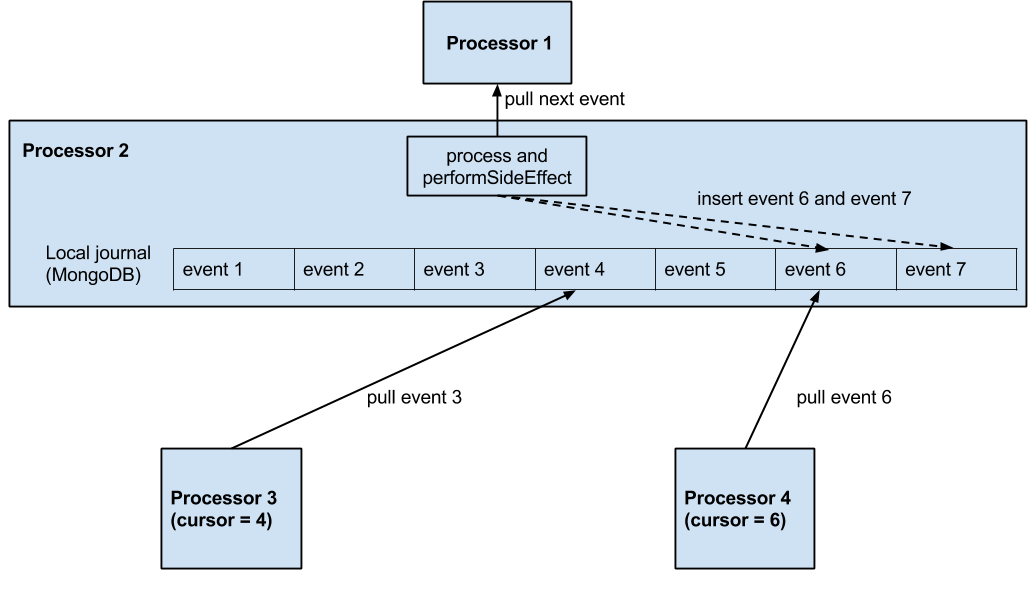
\includegraphics[width=1.0\textwidth]{img/pull_processors.png}}
    \caption{Pull-based streaming}
    \label{fig:pull_processors}
  \end{center}
\end{figure}

With these two functions, fault-tolerance is handled in a clear manner. process is an user-defined function that is the logic of the processor: how to derive one input event to a substream of out events. As a pure function, it is not a problem if it is called several times for the same input. performAtomicSideEffect is then used on each out event to
store it in a local journal. This operation must me \textit{atomic}. Thus, if a processor crashes, when it recovers it just takes the last out event id "LastID" from its local journal and asks its parent for the event that generated the substream containing this out event. The parent re-sends this event which is put again in the process method (at-least-once call semantic). This process method re-creates the substream, and a filter is put on the substream to take only the out events that are \textit{after} the original "LastID" output event. This
filtered substream is then given to the performAtomicSideEffect method that goes on storing events in the local journal as usual. Figure \ref{fig:pull_processors_tolerance} illustrates
the fault-tolerance of event-sourced pull-based processors. TODO EXPLAIN IMAGE

\begin{figure}[h]
  \begin{center} 
    \makebox[\textwidth]{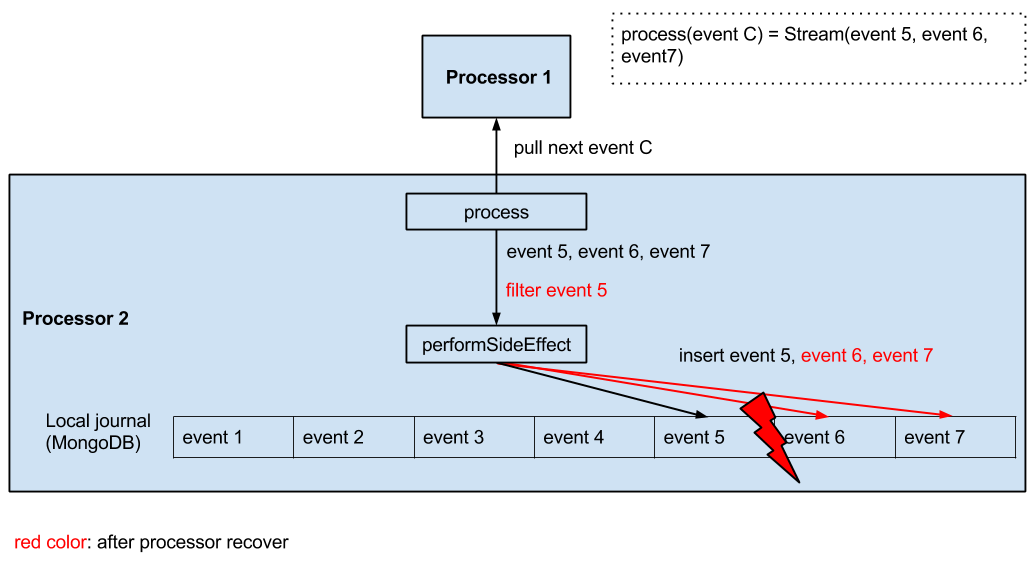
\includegraphics[width=1.0\textwidth]{img/pull_processors_tolerance.png}}
    \caption{Fault-tolerance in event-sourced pull-based processors}
    \label{fig:pull_processors_tolerance}
  \end{center}
\end{figure}

Thus, we have ensured no message loss, no message duplication and guaranteed message ordering in cases of processor crashes. It is easy to see why the "insert in journal" operation in performAtomicSideEffect needs to be atomic: if it is not (say it has 2 steps), if the processor fails between step 1 and step 2, we are in a position where
we don't know if the current out event has been inserted or not where the processor recovers.

This atomicity leads to a potential problem: if we already use the performAtomicSideEffect for inserting output events in the journal, there is no room left for an arbitrary side-effect that can be defined by the user of the library. This is why we define two kinds of processors: \textit{persistent} processors where the performAtomicSideEffect is already implemented to insert output events in a local journal (the type of processor described in this section), and \textit{side-effect} processors that allows to define
an arbitrary atomic side-effect. Side-effect processors will be described in details in section \ref{sec:sideeffectproc}.

Thus, for a persistent processor, the fact that an input event has been "entirely" processed means that all of the out events in the substream it has generated are inserted in the local journal.
\\

One key operation that has not been explained is how to know which input event has generated a particular output event generated in a substream. This is a complex task for which the notion of Path Ids has been created.

\subsubsection{Auto generation of Tree-like Ids: Path Ids}

The generation of events across the tree of processors can be seen itself as an Tree-like structure. For example, when event 1 comes from the Journal and enters in the first
processor, event 1 can generate a substream of events (say event 1-1, event 1-2 and event 1-3). Then, a child processor that generates a 2-event substream
will generate event 1-1-1, event 1-1-2, event 1-2-1, event 1-2-2, event 1-3-1 and event 1-3-2 (see Figure \ref{fig:treepathid}).

\begin{figure}[h]
  \begin{center} 
    \makebox[\textwidth]{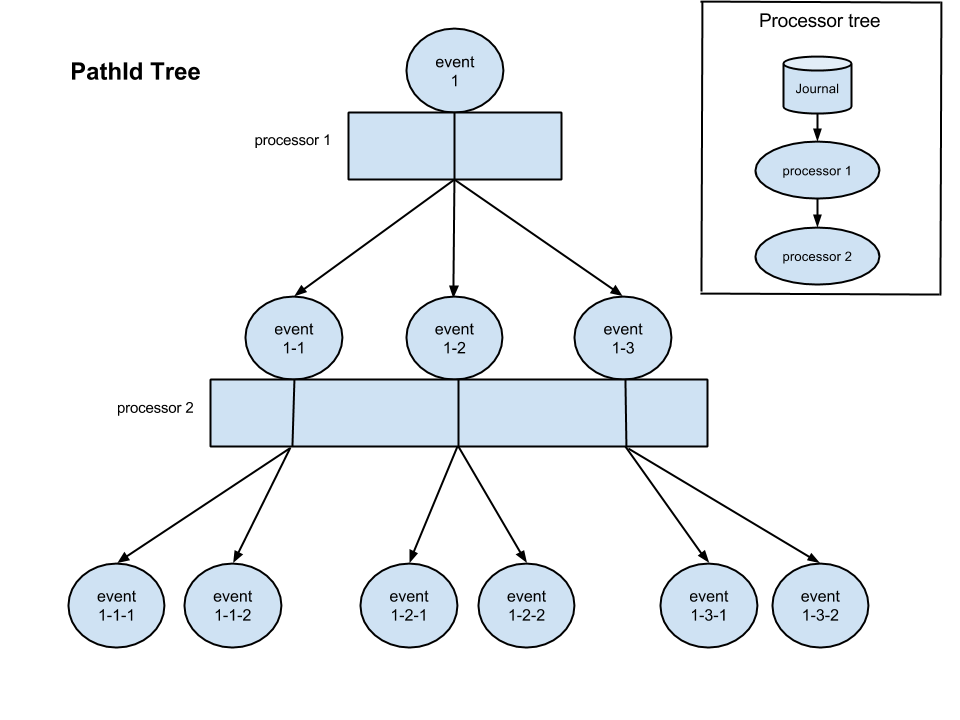
\includegraphics[width=1.0\textwidth]{img/id_tree.png}}
    \caption{A generational tree of PathIds}
    \label{fig:treepathid}
  \end{center}
\end{figure}

We see that the generation of events has a tree-shape, and each event can be characterized by a path in this tree (for example, 1-2-1). The idea of PathId is to
auto-generate these path ids when events pass through processors so that it is possible to re-climb the tree given a particular event.

Concerning fault-tolerance, a child processor that recovers after a crash can check its last PathId, remove the last node "LastNode" of it and send this path id to its parent. Then, the parent sends him the event that the child re-processes (re-creating the substream), and thanks to the number "LastNode" of the last node the child can know from where in the substream it crashed. The idea of id generation to be able to retrieve from a child event the parent event comes from Apache Storm, a distributed and fault-tolerant real-time computation framework \footfullcite{bib:storm}.

The implementation part will explain in more details how these PathIds are serialized and deserialized in MongoDB.

The ability of re-climbing the generational tree is also very useful for side-effect stream processors that are described in the next section.

\subsection{Adaptive push-pull streaming}
\label{sec:adapativepushpull}

An important optimization can still be made to this model. For now, from a processor point of view, receiving input events and sending output events are totally
decoupled tasks that are asynchronous between each others. All input events are processed and the resultant substream is written to the local journal, and then children consume events from this journal. 
If the children were late in the stream, this is the only solution, but if the children were up-to-date in the stream, it would be more performant to just send the processed out events directly to the children (without having them pulling from the local journal of its parent, which involves more IO calls to the local journal).
\\

To do this, a processor maintains a state for each of its children. The state can be UpToDate, WaitingForDownStreamAck or Late.

UpToDate means that the parent knows that its child is up-to-date with the stream, so the out event(s) generated by the next input event that it will receive can 
directly be sent to its child after being inserted in the local journal. Thus, the child does not have to lookup in the journal to get the event (this saves one IO round-trip to the local journal).

WaitingForDownStreamAck is an intermediate step where the parent knows that it has sent an output event to its child, and is waiting for a child ACK meaning that it has
processed the event. Thus, if a new input event comes in when the parent maintains this state
for its child, it means that the child is now Late in the stream, so the parent moves the child's state to Late. If an ACK message comes from the child, the parent moves the
child's state to UpToDate.

Late means that the child is late in the stream, so there is no point sending him the processed out events when a new input event arrives (or it will receive the events out of order).
In this case, the child will replay the stream at its rate. However, if it manages to catch-up with the real-time stream, its state will move to UpTodate.

Figure \ref{fig:childstates} illustrates this as a state transition diagram.

Thus, a processor adapts its stream strategy in real-time between push and pull to optimize performance and latency.

\begin{figure}[h]
  \begin{center} 
    \makebox[\textwidth]{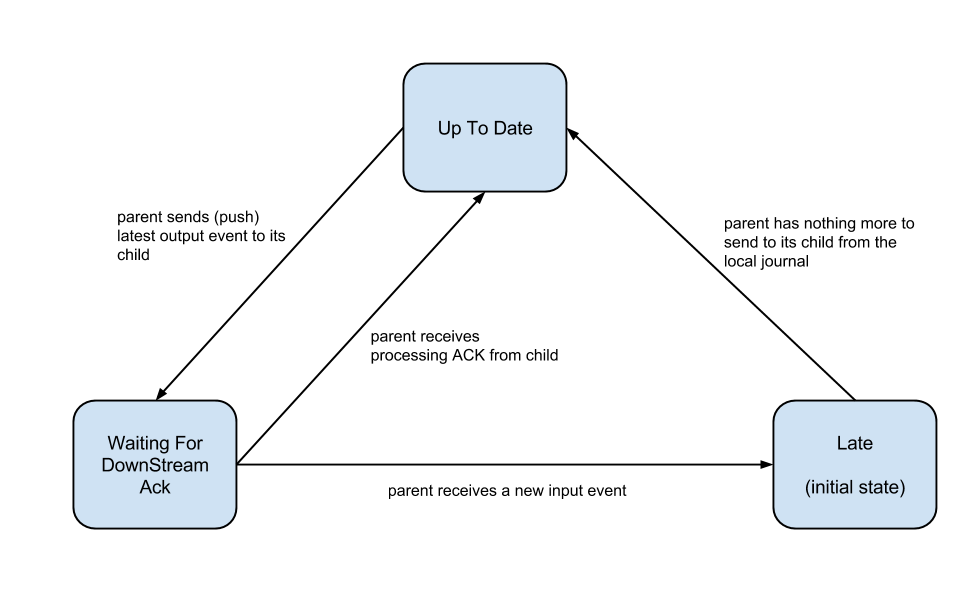
\includegraphics[width=1.0\textwidth]{img/childstates.png}}
    \caption{State transition diagram for each child of a parent processor}
    \label{fig:childstates}
  \end{center}
\end{figure}

\subsection{Side-effect stream processors}
\label{sec:sideeffectproc}

Persistent event-sourced processors use their performAtomicSideEffect method to insert the generated out events in their local journal. We saw that a persistent processor can only do one
atomic side-effect per out event in order to guarantee exactly-once side-effect semantic even in cases of failure. Moreover, a persistent processor uses a lot of disk space as it stores
every output event in its local journal.

To deal with these problems, we define another type of processors: side-effect processors. Side-effect processors do not have a local journal. Instead, when one of its children is slow
and ask for past events, it must ask to its parent to replay these events. However, for children that are up-to-date with the stream, it sends directly the output events to them.

Concerning the replay mechanism for slow children, this is a recursive call until the nearest parent processor that is persistent which is the tree root (Journal) in the worst case. 
Moreover, each intermediate side-effect processor in this recursive call must take care of sending only the minimal amount of messages in substreams. Indeed,
as we re-climb the generational PathId tree, each event sent by a parent is put in the process method of its child that generates the substream. We must just send
events of this substream from a certain event because all events generated from previous events of the substream have already been processed by the original side-effect processor asking for a stream replay. 
Figure \ref{fig:sideeffectreclimb} illustrates this mechanism. TODO explain image

\begin{figure}[h]
  \begin{center} 
    \makebox[\textwidth]{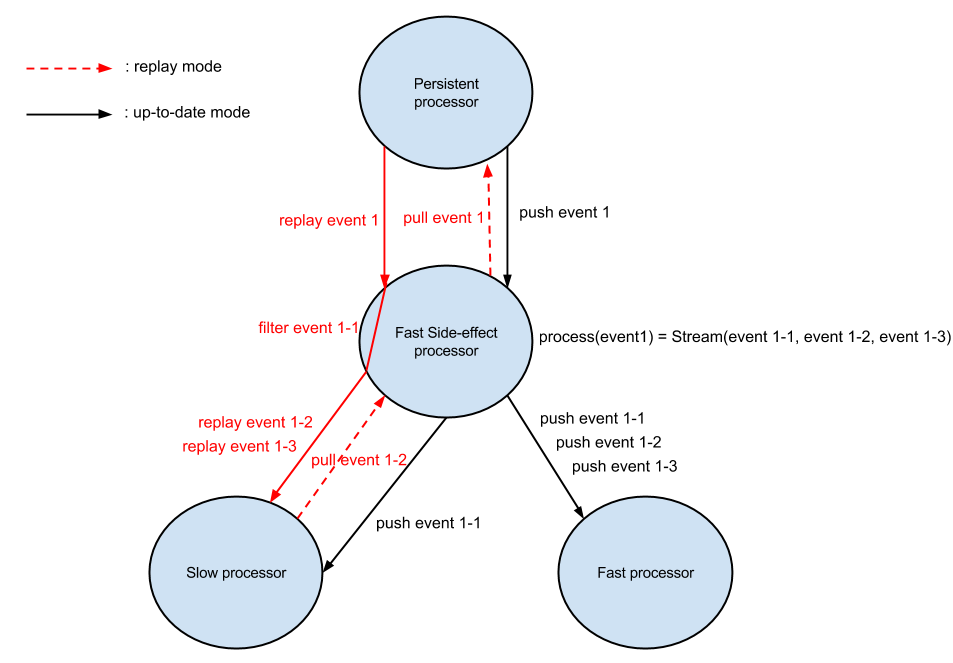
\includegraphics[width=1.0\textwidth]{img/side-effect-reclimb.png}}
    \caption{The stream replay mechanism with side-effect processors}
    \label{fig:sideeffectreclimb}
  \end{center}
\end{figure}

Concerning the performAtomicSideEffect method, the contract for the side-effect is that it has to be atomic if one wants to have the exactly-once side-effect semantic, and moreover the side-effect of an out event should store its PathId somewhere to be able to retrieve it when it recovers from a crash (to keep the fault-tolerance property). Note that this is not the same than inserting the event in a journal as in persistent processors: here we only need to store the latest PathId, not the entire sequence of events. Upon a recover, a method getLastProcessedEventId of signature \verb|getLastProcessedEventId(): Future[PathId]| is able to retrieve the last PathId processed to initiate the recover mechanism explained in the previous section.
\\

In the end, side-effect processors allow to define an arbitrary side-effect (with some constraints), allow to save disk space because it does not maintain
a local journal, but it implies that event stream replays take longer because a side-effect processor cannot replay the stream itself, it has to ask to its parent. However, if a processor is known to produce events slower than its children process them, a side-effect processor is a good trade-off because its "push-mode" is as fast as a persistent processor for up-to-date children.


\subsection{Optimized ACK mechanism with back-pressure using Iteratees}

Concerning the ACK mechanism from a child to its parent, a naive way to do it would be for the child to send an application-level ACK message for each event received and processed. We will take a more performant approach by leveraging the built-in back-pressure mechanism of Iteratees. 

A processor is composed of one Iteratee in input (stream consumer) and several Enumerators (stream producers) in output (one per child). As explained in section \ref{sec:iteratees}, the back-pressure mechanism allows a stream producer to automatically slow down its producing rate if the consumer is slow. 
More precisely, for each child, the "producing" code of it's parent Enumerator will be called to generate the next event only when the consuming Iteratee has totally consumed the current event (like an ACK mechanism). In our case, the Enumerator has the choice to get a stream from the local journal or its parent (Late case), or to directly send the latest output event (UpToDate case).
The Iteratee is the child that receives an event and processes it to create a substream.
Thus, we see that we don't need to create an application-level ACK as the mechanism of notifying the producer when the consumer has finished processing an event is already
built-in in the Iteratee concept. But how does this work in a distributed setting ?


\subsection{Distributed processors with TCP-level back-pressure}

The pipeline composed by an Enumerator (source) and an Iteratee (sink) can be distributed via an HTTP chunked stream. An HTTP chunked stream is a unidirectional stream protocol that allows the producer (server) to maintain a connection with a client to send a possibly infinite number of chunks. An enumerator can be transformed very easily into a HTTP stream producer, and an Iteratee can be easily transformed in a HTTP stream client (more details in the Implementation part). Thus, processors can be distributed via HTTP streams on top of TCP.
\\

By plugging Enumerators / Iteratees via an HTTP stream, one very interesting property is that the back-pressure mechanism remains by leveraging TCP's flow control mechanism. In a few words, if a client does not consume its receive TCP buffer, it will send an ACK message to the sender with a sliding window of size 0, meaning that it does not want more data for now, so the sender stops sending data (this is known as TCP's sliding window flow control protocol).

Thus, Play Framework's Iteratee library leverages this mechanism the propagate back-pressure in a distributed setting. Therefore we have a TCP-level ACK and back-pressure mechanism, which is of course very performant compared to application level ACK messages. Figure \ref{fig:tcpbackpressure} illustrates this concept.

\begin{figure}[h]
  \begin{center} 
    \makebox[\textwidth]{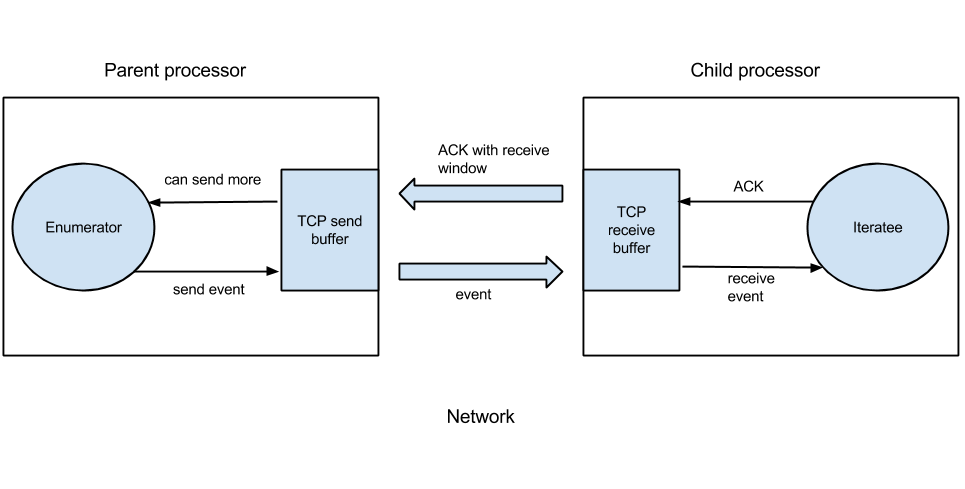
\includegraphics[width=1.0\textwidth]{img/tcpbackpressure.png}}
    \caption{Distributed processors with TCP-level back-pressure}
    \label{fig:tcpbackpressure}
  \end{center}
\end{figure}


\subsection{The Journal: a special case of persistent processor}

The Journal (root of the processing tree) is a particular processor as its source is not a replayable processor. Instead, it has multiple sources: all the pullers from the Data
Integration part that push events concurrently in the Journal. Moreover, its \verb|process| method is the identity function, as the events inserted are the same as the output events.

Concerning the ordering of the events, a particular abstraction from Play Framework Iteratee library is used, called Broadcast Channel, which allows to linearize into a single pipeline events that are pushed from different sources (more details in the Implementation part).

Concerning back-pressure, it depends on the data source if the producer can be slowed down or not. To handle different cases, the Journal has an interface to push events that allows optional back-pressure. Its signature is \textbf{write(event: E): Future[E]}. E is the type of the event. The method returns a Future[E] that will be fulfilled when the event has been inserted in the journal. The event returned in the future in the same event but with a PathId added when it has been inserted in the MongoDB-based journal.
Thus, this Future is like an ACK that the Journal had successfully stored the event. If another event is written \textit{once} this Future has been fulfilled, it is ensured
that this new event will be ordered after the previous event. The future also propagates back-pressure, because if a producer waits for this Future before sending a new event, it means that it has waited that the Journal had time to process it. Producers that can not wait for the Future to be fulfilled can call the \verb|write| method several times
ignoring the Futures returned. However, in this case, there is no guarantee that the event has been correctly inserted, and if all producers act like that the Journal may be overwhelmed. Thus, if possible, it is better to throttle the insertion rate using the Future returned by the write method.

\subsection{Example application}

Using this generic stream processing library, an example application has also been implemented to meet functional business requirements. The aim of this application is to
maintain real-time dashboards on business data (sales, production, finance, ...). Data read latency must be really low, so creating pre-computed dashboards that
update themselves upon the reception of certain kinds of events is an interesting approach. Moreover, upon the reception of some events, the platform should react by updating other external services.
\\

Figure \ref{fig:exampleapp} shows the tree of processors used. 

\begin{figure}[h]
  \begin{center} 
    \makebox[\textwidth]{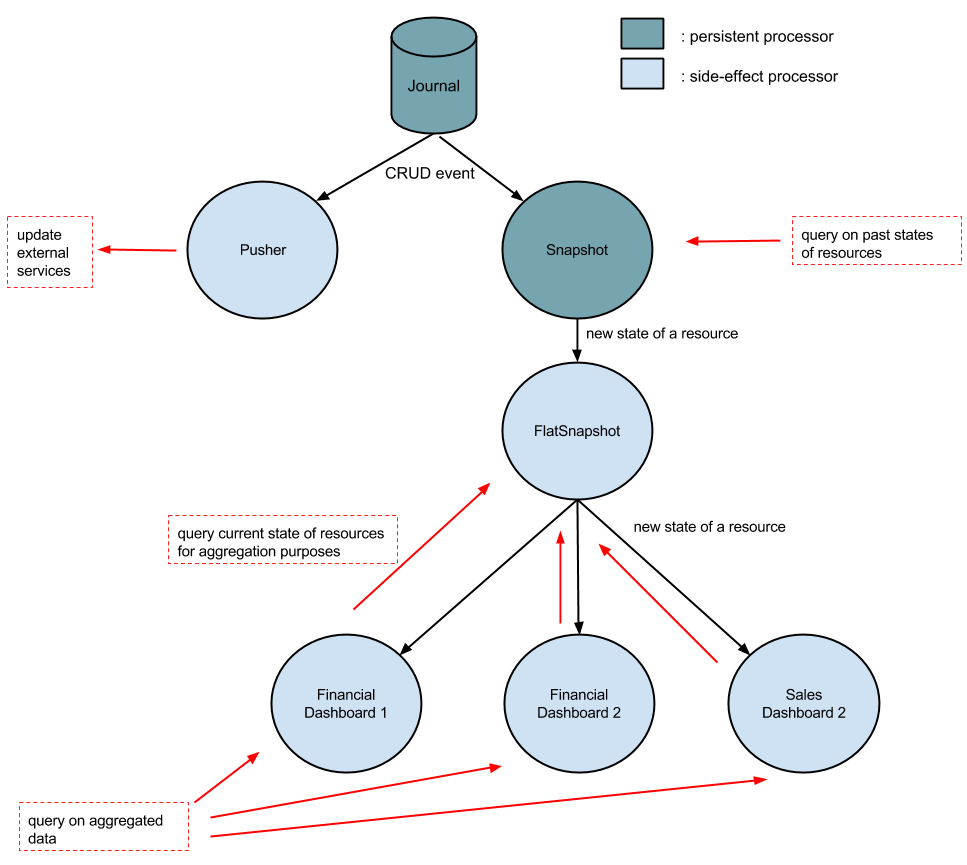
\includegraphics[width=1.0\textwidth]{img/exampleapp.png}}
    \caption{Example application of processors for pre-computed dashboards that update incrementally}
    \label{fig:exampleapp}
  \end{center}
\end{figure}

Snapshot is a persistent processor that maintains the history of all resources (it contains all states of each resource). It takes journal events in input and return the current
state of a resource in output. Its persistent nature allows other services to query its local journal to know past states of resources.

Pusher is a side-effect processor responsible for updating other services upon the reception of particular events. Its side-effect is used to do an in-place update of the last PathId
it has seen.

FlatSnapshot is side-effect processor that uses its side-effect to maintain a MongoDB view on the last state of each resource that is not deleted. Its process method is the identity function on the current state of a resource. 

Dashboards are side-effect processors that use their side-effect to maintain pre-computed aggregation views on various resources. They take the new current state of a resource as input,
and returns a substream of new updated aggregation lines as output.



